%\documentclass[wsdraft]{ws-procs11x85}

\documentclass{ws-procs11x85}
\usepackage{ws-procs-thm}           % comment this line when `amsthm / theorem / ntheorem` package is used
\usepackage{multirow}
\usepackage{tabularx}
\newcommand{\etal}{\textit{et al}.}
\newcommand{\TEtranscripts}{\texttt{TEtranscripts}}
\newcommand{\SalmonTE}{\texttt{SalmonTE}}
\begin{document}

\title{Ultra-Fast and Scalable Quantification Pipeline of Transcript Abundances from Next Generation Sequencing Data}

\author{Hyun-Hwan Jeong$^{1,2}$, Hari Krishna Yalamanchili$^{1,2}$, Caiwei Guo$^{2,3}$,Joshua M. Shulman$^{1,2,3}$, and Zhandong Liu$^{2,3,\dag}$}

\address{$^{1}$Department of Molecular and Human Genetics, Baylor College of Medicine,\\
$^{2}$Jan and Dan Duncan Neurological Research Institute, Texas Children’s Hospital,\\
$^{3}$Department of Neuroscience, Baylor College of Medicine,\\
$^{4}$Department of Pediatrics, Baylor College of Medicine,\\
Houston, Texas 77030, USA\\
$^{\dag}$E-mail: zhandonl@bcm.edu}

\begin{abstract}
Transposon elements (TE) are DNA elements which have mobility and represent a large proportion (45\%).
Most of them are not functional, but some of them can be causes of genetic disease. 
Rapid development of RNA-seq generates a big genomic data repository and gives a chance for a large-scale study for TE, but 
% * <phamkala@gmail.com> 2017-07-28T18:24:56.789Z:
% 
% > for
% Replace "for" with "of"
% 
% ^ <jeonghyunhwan@gmail.com> 2017-07-28T22:16:04.122Z.
% * <phamkala@gmail.com> 2017-07-28T18:23:21.603Z:
% 
% > of 
% Replace "of" with "for"
% 
% ^.
% * <phamkala@gmail.com> 2017-07-28T18:22:41.759Z:
% 
% Instead of "of" use "for"
% 
% ^ <jeonghyunhwan@gmail.com> 2017-07-28T22:17:16.058Z:
% 
% Kala, did you change it already, if you didn't then could you change it? I can't find where you pointed out.
%
% ^ <jeonghyunhwan@gmail.com> 2017-07-28T22:18:43.088Z:
% 
% I think it must be "Rapid development of RNA-seq generates a big genomic data repository and gives a chance for a large-scale study for TE, but ", right?
%
% ^.
no feasible TE analysis tools are out yet.
In this work, we have developed \SalmonTE, a fast and reliable pipeline for quantification of TEs from 
Next Generation Sequencing (NGS) data.
% * <phamkala@gmail.com> 2017-07-28T18:26:23.109Z:
% 
% > NGS
% Not sure if you specified early, but what is NGS? Does it stand for Next Generation Sequencing Data? If so,  replace "NGS" with "Next Generation Sequencing  (NGS)" so that it is clear. After this, you can use NGS wherever you want and it will be clear that you are talking about Next Generation Sequencing. 
% 
% ^ <jeonghyunhwan@gmail.com> 2017-07-28T22:14:55.653Z:
% 
% It is fixed. Thanks.
%
% ^.
The demonstration of \SalmonTE~for the various datasets has shown a dramatical speed-up compared to \TEtranscripts, 
% * <phamkala@gmail.com> 2017-07-28T20:11:31.823Z:
% 
% > the
% Change to "a"
% 
% ^.
% * <phamkala@gmail.com> 2017-07-28T20:08:50.667Z:
% 
% > comparing
% Change to "compared"
% 
% ^.
and the comparison of counts and fold-changes to the previous method and RT-qPCR has shown this pipeline can 
provide an precise quantification result for a given input dataset. 
% * <phamkala@gmail.com> 2017-07-28T20:12:00.410Z:
% 
% Maybe add "a" before "given"
% 
% ^.
We conclude this pipeline will be the first starting point which enables a large-scale TE study.
\end{abstract}

\keywords{Transposon Element; Quasi Mapping; RNA-seq; Next Generation Sequencing; Large Scale Genome Analysis}

% required
\copyrightinfo{\copyright\ 2017 The Authors. Open Access chapter published by World Scientific Publishing Company and distributed under the terms of the Creative Commons Attribution Non-Commercial (CC BY-NC) 4.0 License.}

% required
\bodymatter

\section{Introduction}\label{aba:intro}

Transposon elements (TE) are DNA elements which can be mobilized or inserted in the genome and represent a significant proportion (45\%) of most eukaryotic genomes \cite{erwin2014mobile}. 
% The first observation of TEs was in \textit{Zea Mays (maize)} by Barbara McClintock in 1948 \cite{McClintock01011951}. 
Most of the TEs in genome are not functional and had been considered as `junk DNA,' but some of the TEs have functions such as transcription and mobilization.\cite{biemont2006genetics}
Furthermore, TEs are able to be mutagens, and their mobilization can be a cause of genetic disease \cite{belancio2008mammalian} such as cancer,
\cite{jirtle2007environmental}
neurodegenerative diseases,\cite{erwin2014mobile} and aging.\cite{wood2013chromatin} % citations!

Recent development of high-throughput Next Generation Sequencing (NGS), like RNA-seq
enables a genome wide study for TEs\cite{ohtani2013dmgtsf1,mihevc2016tdp,li2012transposable,krug2017retrotransposon}, and several algorithms and pipelines were proposed to analysis reads files from TE studies \cite{lee2012landscape,platzer2012te,helman2014somatic,henaff2015jitterbug,jin2015tetranscripts,de2017identifying}. However, most of the tools have several issues: Discordant read mapping issue, due to chance of multiple mapping, limited scalability of large-scale analysis, and some tools are limited because these tools only consider a specific type of TE.
\cite{ewing2015transposable} 
Among those previous tools, \TEtranscripts~is a tool resolve most of the issues and has shown it performs accurately for various datasets.
\cite{jin2015tetranscripts}
Nonetheless, The scalability of \TEtranscripts~is still limited because this tool cannot handle \verb|FASTQ| file directly and needs to generate \verb|SAM|(Sequence Alignment Map)/\verb|BAM| (Binary Sequence Alignment Map) files from raw \verb|FASTQ| files to execute \TEtranscripts, and this step might take a long time and aggravate computational burden.
Furthermore, the interval tree algorithm \cite{samet1990design}, which is used to find interval of genes or TEs on reference genome, which is corresponded given alignment results does not practically perform faster than the expectation. Thus, \TEtranscripts~is not a feasible tool to perform large-scale TE analysis.

Although most of TE studies contains a few of RNA-seq samples, recent studies demonstrated that large-scale analysis of public RNA-seq 
datasets offers a robust analysis of the interests and observed novel 
findings which were not observed before. \cite{nellore2016human} There is no doubt that a study of TE with a large-scale analysis with NGS dataset can give us a novel point of view for TE. To enable this, we have developed an alternative pipeline of \TEtranscripts, \SalmonTE. It deploys quantification methods of \verb|Salmon|\cite{patro2017salmon} and contains various statistical analysis for the quantifications. Moreover, user do not have to do any pre-processing for their raw \verb|FASTQ|. 
With experiments in this work, we show running speed \SalmonTE~outperforms \TEtranscripts~and gives a reliable quantification result of \SalmonTE~from different public datasets.

\section{Methods}

The proposed pipeline consists of three parts: Transposon element library preparation, quantification, and statistical analysis. Fig. \ref{aba:fig1} introduces how this proposed pipeline works.
The entire source codes and executable scripts are available at \url{https://github.com/hyunhwaj/SalmonTE}. We describe details of the pipeline in this section. 
% Is it better to say "three parts" than "two parts?"

\begin{figure}[!ht]
\centerline{
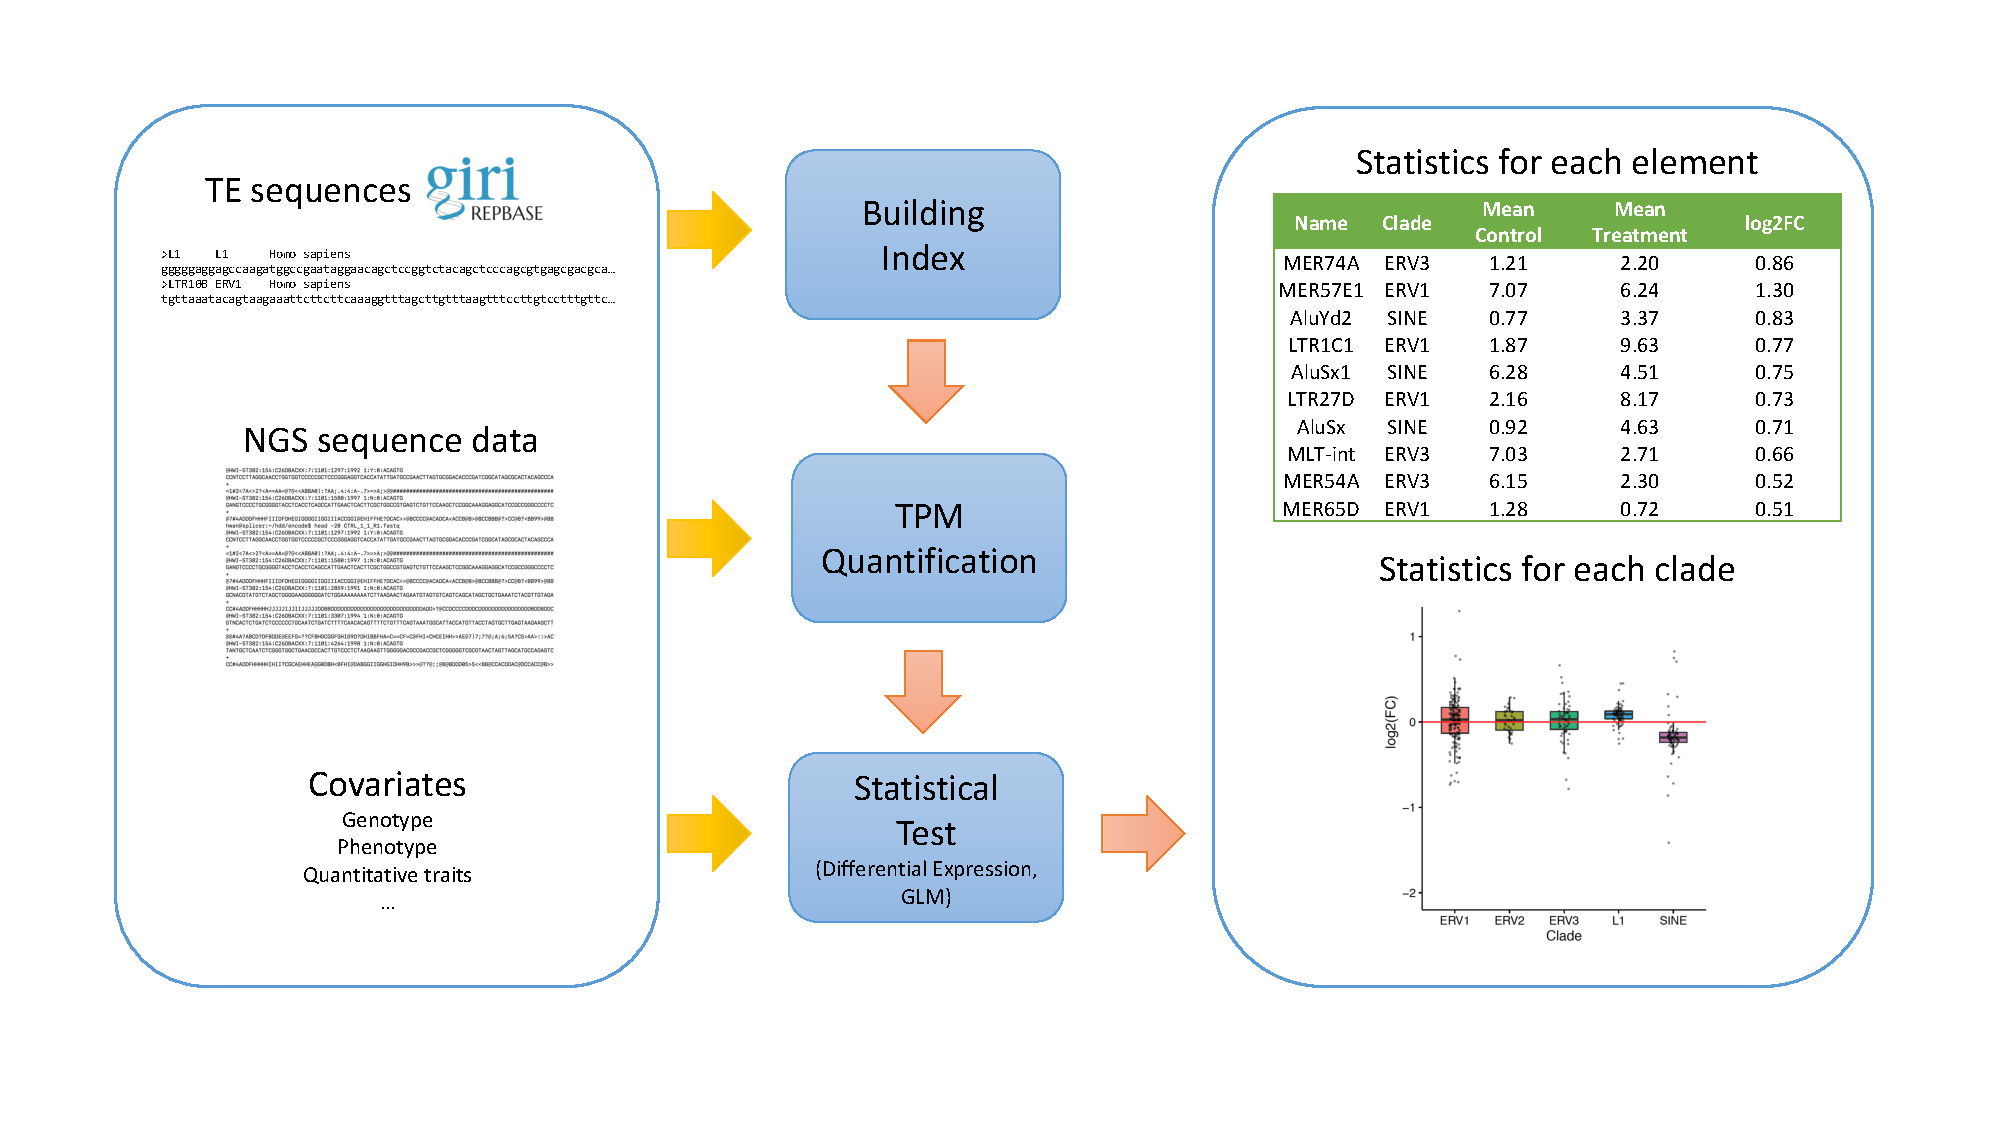
\includegraphics[width=16cm]{fig1.pdf}
}
\caption{An illustration of the \SalmonTE~pipeline}
\label{aba:fig1}
\end{figure}

\subsection{Transposon Element Library Preparation}
The first required data of \SalmonTE~is collecting cDNAs (complementary DNA) of TEs given specie for the quantification.
We collected the consensus cDNA sequence library of TEs for \textit{Homo Sapiens} and \textit{Drosophila Melanogaster} from Repbase  
(version 22.06)\cite{repbase}. We did not include cDNA sequences of simple repeats and multicopy genes, and DNA transposons (which replicate without an RNA intermediate). 
Once we collected the library, we manually curated clades of each TE, based on the annotation of Repbase. As a result, we have 687 TEs for \textit{Homo Sapiens} and 163 TEs for \textit{Drosophila Melanogaster}.
% need to add a table to summarize? We don't have the curated data of DM yet, better to ask Caiwei?

\subsection{Salmon quantification algorithm}

We deploy Salmon\cite{patro2017salmon} to quantify the transposon elements abundance from given RNA-seq reads files. Salmon enables a fast and accurate quantification of transcript expression from RNA-seq reads with quasi-mapping, a variant of stochastic, collapsed variational Bayesian inference(in the online phase), and Expectation Maximization (EM) algorithm (in the offline phase)
\cite{patro2017salmon,srivastava2016rapmap,bishop2006pattern,foulds2013stochastic}. 
We describe details of algorithms and models uses in \verb|Salmon| in this section.

Before running online and offline inference of counts of each transposon elements from given reads file,
Salmon runs a quasi-mapping which has been initially proposed in \cite{srivastava2016rapmap}. A quasi-mapping specifies the target of each given read and also determines the position and the orientation of the read concerning the target by the computation of 
Maximum Mappable Prefix (MMP) \cite{li2012exploring} and Next Informative Position (NIP) \cite{srivastava2016rapmap} of the read.
This mapping procedure depends on a generalized suffix array \cite{manber1993suffix}, 
and it enables a fast and accurate mapping to compare other mapping tools, such as \verb|Bowtie 2|, \verb|STAR|, and \verb|Kalisto| \cite{srivastava2016rapmap}. 

The online phase is to  to model the conditional probability $Pr \{f_j | t_i \}$, and
uses the following auxiliary terms:

\begin{equation}
Pr \{f_j | t_i \} = Pr \{ l | t_i \} 
\cdot Pr \{ l | t_i \} 
\cdot Pr \{ p | t_i, l \} 
\cdot Pr \{ o | t_i \} 
\cdot Pr \{ a | f_j, t_i, p, o, l \} 
\end{equation}

% better to rephrase
where $Pr \{ l | t_i \}$ 
is the probability of drawing a read of the inferred length $l$ given $t_i$,  
$Pr \{ p | t_i, l \}$ is the probability of the read starting at position $p$ on $t_i$,
$Pr \{ o | t_i \}$ is the probability of obtaining a read
alignment with the given orientation $o$ to $t_i$, and
$Pr \{ a | f_j, t_i, p, o, l \} $ is the probability of the alignment $a$ \cite{patro2017salmon}. 
This model accounts for sample-specific parameters and biases.
Laissez-faire stochastic variational Bayes SCVB0 inference algorithm is used to 
Compute the online abundance estimates auxiliary model parameters\cite{patro2017salmon}.

After we had a mapping result of the reads with the procedure and finished the online inference phase, 
we can estimates abundance (reads count) of each transcript with the result. Suppose that
we have $M$ transcripts (TEs in this work) and the set of underlying true transcripts counts are given as
$T = \{(t_1, \dots , t_M), (c_1, \dots, c_M) \}$, where $t_i$ is the nucleotide sequence of $i$-th transcript in the set and $c_i$ is true count of the corresponded transcript. 
If $T$ contains a complete counts then we can calculate the nucleotide fraction \cite{li2009rna} of each $t_i$ from (\ref{eq:1}).
 

\begin{equation} \label{eq:1}
\eta_i = \frac{c_i \cdot \widetilde{l_i} }{\sum_{j=1}^{M} c_j \cdot \widetilde{l_j}}
\end{equation}

In (\ref{eq:1}), let $\widetilde{l_i}$ denote the effective transcript length of $t_i$\cite{li2009rna}.

We also can calculate the transcript fraction of each transcript from (\ref{eq:2}).

\begin{equation} \label{eq:2}
\tau_i = \frac{ \frac{\eta_i }{\widetilde{l_i}} }
{\sum_{j=1}^{M} \frac{\eta_j }{\widetilde{l_j}} }
\end{equation}

$\tau_i$ can be used a measure of relative transcript abundance.

With $\tau_i$, Transcripts Per Million (TPM) calculated as $TPM=\tau_i \times 10^6$ and the $TPM$ uses as a relative abundance measure of each transposon element for a given sample in this study.

To estimate $T$, the maximum likelihood approach is used to assess given $T$ and $F$ which is a given set of mapped sequence reads from 
the online inference step.
We can define the probability of observing a set of sequenced fragments as below,

\begin{equation} \label{eq:3}
Pr\{F|\eta,Z, T \}=
\prod_{j=1}^{N}\sum_{i=1}^{M} Pr\{ t_i | \eta \}  \cdot
 Pr \{ f_i | t_i , z_{ij} = 1 \}
\end{equation}

where $z_{ij} = 1$ denotes if $j$-th read in $F$ is derived from transcript $i$. The likelihood objective can be optimized using EM algorithm \cite{li2009rna}.

To facilitate running this step easier and to ease to enable parallel processing for multiple RNA-seq reads files, we adopted \verb|Snakemake| workflow system and wrote a script of the execution rule for the system.\cite{koster2012snakemake}
% Still completing pipeline, and it will out to github and our website.

\subsection{Statistical tests}

With the covariates data for given samples in the experiments, 
we perform a statistical analysis between quantified TE abundance and the covariate as the last step of the pipeline. 
Differential analysis using DEseq2 can perform for binary covariates such as binary genotype, phenotype and gender \cite{love2014moderated}. We can also apply General Linear Model (GLM) for quantitative covariates such as disease pathology score and age \cite{johnston1980multivariate}. The analysis will make two different outputs, 
the first one is the statistics for each TE, and the second one is the summary of the statistics for each clade. 
The output files are provided with various file formats, such as tab-separated values file (TSV), XML spreadsheet file format (XLS, XLSX), R object file (Rdata), and Portable Document Format (PDF) file.

\section{Results}

\subsection{Experiment setup}
In the paper of \TEtranscripts, they demonstrated that \TEtranscripts~is the best method among the published methods in terms of recovery accuracy of TE and running time for both cases of a synthetic dataset and published data. 
Thus, we only compare performance of our pipeline to \TEtranscripts. 
Ohthani \etal's RNA-seq data from Gene Expression Omnibus (accession no. GSE47006), which were used in the \TEtranscripts~paper, 
were used to compare performance of running time and quantification accuracy between
our proposed pipeline and \TEtranscripts. \cite{ohtani2013dmgtsf1}
As a pilot study, to seek which TEs can differentially express between ALS(Amyotrophic Lateral Sclerosis) human patients and healthy people, 
we demonstrated our pipeline with a K562 cell-line RNA-seq dataset from ENCODE (Encyclopedia of DNA Elements, \url{http://encodeproject.org}) \cite{encode2012integrated} Consortium (accession ID: ENCBS555BYH). 
The dataset consists of two biological replicates of shRNA(short hairpin RNA) knockdown (KD)
which the shRNA targets TARDBP (TAR DNA Binding Protein, as known as TDP-43) gene and two biological replicates of controls 
(a shRNA inserted but targets no genes). 
There are two reasons why we choose the dataset
the dataset because K562 cell-line can be used for the neurodegenerative 
disease studies,\cite{haney2017crispr}
and it was reported that loss of TDP-43 function causes phenotypes of 
ALS.\cite{yang2014partial,mihevc2016tdp} To measure scalability with the dataset
we also ran \TEtranscripts~to compare running time of both methods.


Generating BAM files from \verb|FASTQ| files are mandatory to use \TEtranscripts, so we applied \verb|STAR|\cite{dobin2013star} to generate the files with following parameters
\verb|--outFilterMultimapNmax 100| and \verb|-–winAnchorMultimapNmax 100|. We also used 16 threads for the both \SalmonTE~and \verb|STAR|(for \TEtranscripts).
All of computational experiments in this work had performed in a workstation with 
\verb|Intel(R) Xeon(R) CPU E5-2630 v4 @ 2.20GHz| (has 10 cores and maximum 40 threads) and \verb|128GBytes| RAM.


\subsection{Performance Benchmarking of \SalmonTE}

Table \ref{aba:table1} shows a summary of the datasets used in the experiments and indicates the result of measuring the runtime of \SalmonTE~and \TEtranscripts~for both datasets. 
The results show the speedup of \SalmonTE~factors between 19.00 and 27.28,
regarding comparison with \TEtranscripts. % Hwan: is it okay to say that?
From the comparison, we can conclude that \SalmonTE~outperforms \TEtranscripts~regarding processing speed, and this pipeline just took less than 5 minutes for a sample, while \TEtranscripts~needs to take about 2 hours to proceed each sample. 
It also shows \SalmonTE~has a high potential which enables to have several advantages if the pipeline is extended to a cloud service. 
Table \ref{aba:table_amazon} shows that
Our estimation of running price of the proposed pipeline in the cloud computing environment, and it predicts the price is less than 22 times less than \TEtranscripts.  

\begin{table}[h]
\tbl{Performance comparison between \SalmonTE~and \TEtranscripts}
{
\begin{tabular*}{.8\textwidth}{@{\extracolsep{\fill}}llll}
\hline
Dataset                          & Piwi KD [Refs.~\refcite{ohtani2013dmgtsf1}]    & K562 TDP-43 \\ \hline
Total number of samples          & 2          & 4             \\ 
RNA-seq file type                & Single end & Paired ends  \\ 
Total number of reads            & 90,411,467 & 309,701,182   \\ \hline
\SalmonTE~runtime (hh:mm:ss)      & 0:05:33    & 0:17:13       \\
\TEtranscripts~runtime (hh:mm:ss) & 1:45:26    & 7:49:40       \\
Speedup                          & 19.00x     & 27.28x        \\ \hline
\end{tabular*}}\label{aba:table1}
\end{table}

\begin{table}[h]
\tbl{Price estimation of both \SalmonTE~and \TEtranscripts~in cloud computing environment (Amazon Elastic Compute Cloud (EC2),
and Amazon Elastic Block Store (EBS)). We assume that size of \texttt{FASTQ} file for a sample is 20GB for the calculations.}
{\begin{tabular}{lrr}
\hline
Methods & \SalmonTE~& \TEtranscripts \\ \hline
Estimated total running time for 1000 samples & 90 hours & 2,000 hours \\ 
The price of Amazon EC2 (m4.10xlarge, US Oregon region) [Refs.~\refcite{ec2}] & \$180 & \$ 4,000 \\
The price of Amazon EBS (gp2 40TB, US Oregon region) [Refs.~\refcite{ebs}] & \$500 & \$ 11,111 \\  
Total price & \$680 & \$ 15,111 \\ \hline
\end{tabular}}\label{aba:table_amazon}
\end{table}

\subsection{Quantification}

\begin{figure}[h]
\centerline{
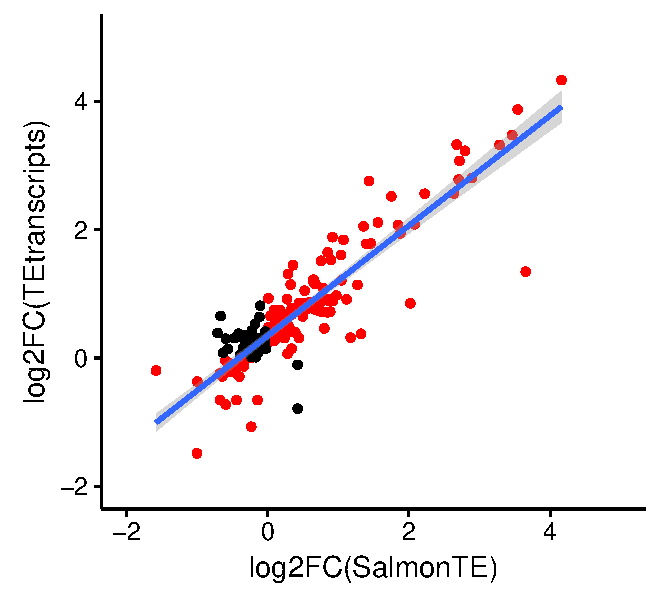
\includegraphics[width=11cm]{figure_corr_FC}
}
\caption{Correlation of $log_{2}FC$ ($\frac{Piwi}{WT}$) for each transposon element between \SalmonTE~and \TEtranscripts. Red points represents points shows same sign of estimated $log_{2}FC$ from \SalmonTE~and \TEtranscripts.}
\label{aba:fig2}
\end{figure}

We firstly compared estimated $log_{2}FC$ of \SalmonTE~and TETranscripts for each transposon element from Ohtani \etal's data. 
Fig. \ref{aba:fig2} shows that the estimation of both methods are highly correlated ($r^{2}=0.98$), and we can observe there is a high concordance direction of fold-changes between \SalmonTE~and TETranscripts. We also measured the correlations of normalized reads count between \SalmonTE~and \TEtranscripts, 
and we can see that the calculated read counts from those methods are highly correlated for each sample. ($r^2=0.92$ for wild-type (WT) sample and $r^2=0.91$ for PiWi KD sample).
From this observation, we can expect that \SalmonTE~is considered as the pipeline which can produce accordant results of \TEtranscripts.

\begin{figure}[h]
\centerline{
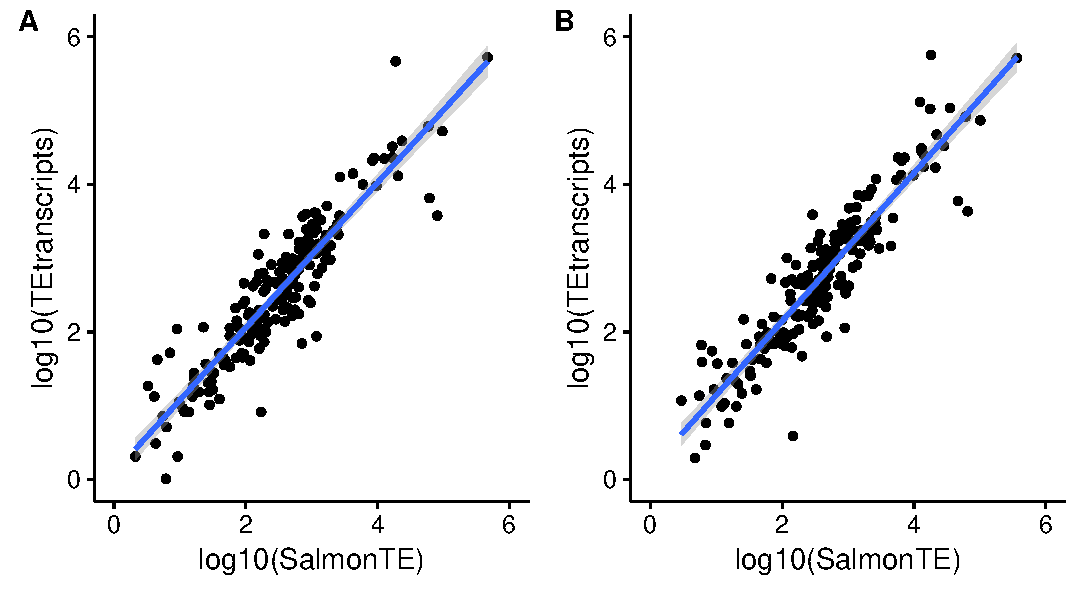
\includegraphics[width=13cm]{figure_corr_count}
}
\caption{Sample correlation of count for each transposon element between \SalmonTE~and \TEtranscripts. \textbf{A}. WT sample, \textbf{B}. PiWi KD sample.}
\label{aba:fig3}
\end{figure}

We nextly took 8 TEs which were quantified by RT-qPCR
(The Reverse Transcription Quantitative Polymerase Crain Reaction)
and validated with measuring the correlation of $log_{2}FC$ of each selected TE between RT-qPCR and \SalmonTE.
As Fig. \ref{aba:fig4} shows, there is a high correlation between \SalmonTE~and RT-qPCR for those elements ($r^2=0.97$), and we can conclude
\SalmonTE~estimate $log_{2}FC$ substantially from the qPCR validation result.

\begin{figure}[h]
\centerline{
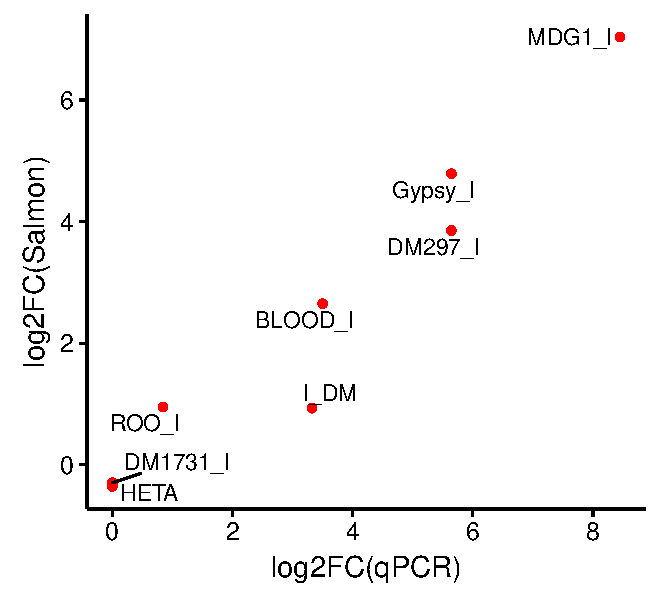
\includegraphics[width=10cm]{supp_fig3_corr}
}
\caption{Comparison between \SalmonTE~and RT-qPCR}
\label{aba:fig4}
\end{figure}

\subsection{Demonstration on K562 cell-line TDP-43 data}

Finally, we applied \SalmonTE~pipeline to a TARDBP(TAR DNA Binding Protein, as known as TDP-43) knockdown human-cell line RNA-seq data to see whether we find novel differentially expressed transposon elements and clade. 
Table \ref{aba:table2} contains list of 23 transposon elements shows differential expressions between TARDBP knockdown cell-line
samples and control cell-line samples. $|log_{2}FC| \geq 0.5$ was used as the threshold of differential expression of transposon elements. We can see that most of the differentially expressed features are Endogenous Retrovirus (15 of 23) in TDP-43 cell-line sample, and 
we presume that some of differentially Endogenous Retrovirus TEs are associated with ALS.

% we may need to the interpretation

We also sought whether there are any general trends of differential expression for each clade. 
In the analysis, all of the CR1 (Chicken Repeat 1) were discarded because the number of elements in the clade is small.
We found that SINE (Short Interspersed Nuclear Elements) are mostly down expressed,
and elements in L1 (Long interspersed nuclear element 1) are over expressed in TARDBP knockdown samples. 
This result gives a conclusion that knocking-down of TDP-43 arises overall less expression of SINE elements and higher expression of L1 elements.

\begin{table}[h]
\tbl{23 Differentially expressed transposon elements in the ENCODE TARDBP data}{
\begin{tabular*}{.5\textwidth}{@{\extracolsep{\fill}}ccc}
\hline
Name & Clade & log2FC\\
\hline
MER74A & ERV3 & 1.68\\
MER57E1 & ERV1 & 1.30\\
AluYd2 & SINE & 0.83\\
LTR1C1 & ERV1 & 0.77\\
AluSx1 & SINE & 0.75\\
LTR27D & ERV1 & 0.73\\
AluSx & SINE & 0.71\\
MLT-int & ERV3 & 0.66\\
MER54A & ERV3 & 0.52\\
MER65D & ERV1 & 0.51\\
LTR28 & ERV1 & -0.59\\
LTR1F & ERV1 & -0.63\\
FLAM & SINE & -0.64\\
MER21 & ERV3 & -0.68\\
MER101 & ERV1 & -0.69\\
LTR26B & ERV1 & -0.70\\
MER83C & ERV1 & -0.71\\
AluJo & SINE & -0.72\\
LTR06 & ERV1 & -0.73\\
MLT2D & ERV3 & -0.78\\
AluYf5 & SINE & -0.86\\
AluYd3 & SINE & -1.41\\
THER2 & SINE & -2.03\\ \hline
\end{tabular*}}\label{aba:table2}
\end{table}


\begin{figure}[h]
\centerline{
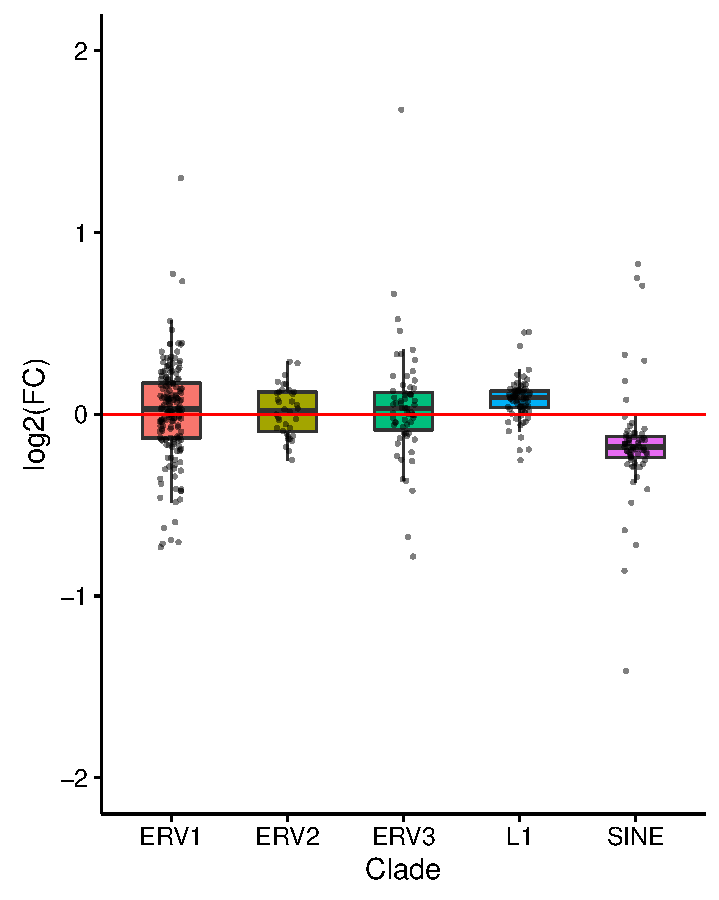
\includegraphics[width=10cm]{boxplot-clade-k562}
}
\caption{An boxplot of $log_{2}FC$ for each clade in the ENCODE TARDBP data}
\label{aba:fig5}
\end{figure}

\section{Conclusion}


In this work, we have developed \SalmonTE, a fast and reliable pipeline for quantification of TEs from 
NGS data.
The demonstration of \SalmonTE~for the various datasets has shown the dramatical speed-up comparing to \TEtranscripts, 
and comparison of counts and fold-changes with a previous method and RT-qPCR has shown this pipeline can give 
a reliable quantification result for the datasets used in the experiment. 
Therefore, we expect this pipeline enables a large-scale TE study.

There are still several tasks need to consider in the future to improve the study of TE. Prediction of genomic locations which 
contain any differential TE expressions can be the most prioritized task among the future works. Several methods for the prediction is
developed \cite{de2017identifying,criscione2014transcriptional}, but these tools have an issue of the scalability and require
massive computing power to do a large-scale TE study. We
anticipate developing a novel pipeline for the prediction with alignment free quantification manner which uses in \SalmonTE~
resolves the issue, but currently developed alignment-free methods such as \verb|Sailfish| \cite{patro2014sailfish}, \verb|Salmon|\cite{patro2017salmon}, 
and Kalisto \cite{bray2015near} are limited to use
because the genomic information of TEs is not prior information to be considered in those methods.
Therefore, we foresee it will need to design a novel algorithm which extends and improve a current alignment-free method.

\bibliographystyle{ws-procs11x85}
\bibliography{ws-pro-sample}

\end{document}